\section{Wasserstein GAN}

In many cases, the GAN algorithm can be thought of as minimizing a divergence between a data distribution 
$p_{\text{data}}(\bm{x})$ and the model distribution $p_{\theta}(\bm{x})$. For example, the minimax GAN discussed 
in the lectures minimizes the Jensen-Shannon divergence, and the loss in problem 3c minimizes the KL divergence. 
In this problem, we will explore an issue with these divergences and one potential way to fix it. Note that for subproblems
(a) to (d), $x$ is not bolded denoting a scalar. This is because $\theta \in \Re$ suggests that we are working with a 
single-variable gaussian distribution.

\begin{enumerate}[label=(\alph*)]
    \item \input{05-wgan/01-kl}

    \item \input{05-wgan/02-kl-limit}

    \item \input{05-wgan/03-alt}

    \item \input{05-wgan/04-alt-limit}

    \item \points{5e} The Wasserstein GAN with gradient penalty (WGAN-GP) enables stable training by penalizing functions whose 
    derivatives are too large. It achieves this by adding a penalty on the 2-norm of the gradient of the discriminator 
    at various points in the domain. It is defined by

    \begin{equation} \label{eq:24}
        L_D(\phi; \theta) = \E_{\bm{x} \sim p_{\theta}(\bm{x})}[D_{\phi}(\bm{x})] - \E_{\bm{x} \sim p_{\text{data}}(\bm{x})}[D_{\phi}(\bm{x})] + \lambda \E_{\bm{x} \sim r_{\theta}(\bm{x})}[({\left\| \nabla D_{\phi}(\bm{x})\right\|}_{2}-1)^2]
    \end{equation}

    \begin{equation} \label{eq:25}
        L_G(\theta; \phi) = - \E_{\bm{x} \sim p_{\theta}(\bm{x})} [D_{\phi}(\bm{x})]
    \end{equation}

    where $r_{\theta}(\bm{x})$ is defined by sampling $\alpha \sim \text{Uniform}([0,1])$, $\bm{x}_1 \sim p_{\theta}(\bm{x})$, and
    $\bm{x}_2 \sim p_{\text{data}}(\bm{x})$, and returning $\alpha \bm{x}_1 + (1-\alpha)\bm{x}_2$. The hyperparameter $\lambda$ 
    controls the strength of the penalty; a setting that usually works is $\lambda = 10$. Also note that ${\left\| \nabla D_{\phi}(\bm{x})\right\|}_{2}$
    is the Frobenius norm.

    Implement and train WGAN-GP for one epoch on Fashion MNIST. In \texttt{submission/gan.py}, implement the 
    \texttt{loss\_wasserstein\_gp\_g} and \texttt{loss\_wasserstein\_gp\_d} functions. 
    
    To train the model, execute:
    \begin{verbatim}
        python main.py --model gan --out_dir gan_wass_gp --loss_type wasserstein_gp
    \end{verbatim} 

    For GPU acceleration run run the command below. \textbf{Note:} we are not supporting MPS GPUs as it trains slower than CPU-enabled training on Apple Silicon devices.
    \begin{verbatim}
        python main.py --model gan --out_dir gan_wass_gp --loss_type wasserstein_gp --device gpu
    \end{verbatim} 
    
    You may monitor the GAN's output in the \texttt{gan\_wass\_gp} directory. The generated images should resemble the image below:

    \begin{figure}[h]
        \centering
        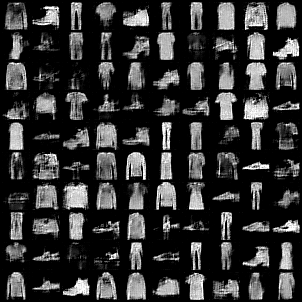
\includegraphics[width=0.5\textwidth]{./figures/gan_wass_gp_0900}
    \end{figure}

    \textbf{Hint: }Avoid using for loops and try a vectorized approach. For the vectorization, consider if you can get a 
    common term, such that differentiating that term with respect to $x^{(i)}$ gives you the required gradient for that input.

    We are trying to obtain the following matrix of derivatives 
    (we will then take the norm of each row, for use in the gradient penalty): 

    \begin{center}
       
        \[
            \texttt{grad} =
            \begin{bmatrix}
                \frac{\partial D(\bm{x}^{(1)})}{\partial \bm{x}^{(1)}} \\
                \vdots \\
                \frac{\partial D(\bm{x}^{(m)})}{\partial \bm{x}^{(m)}} \\
            \end{bmatrix}
        \]
    \end{center}

    In principle, we could compute $\frac{\partial D(\bm{x}^{(i)})}{\partial \bm{x}^{(i)}}$ using a \texttt{for} loop 
    over each element in the batch and then stack the resulting derivates. However, this is inefficient. Instead notice that

    \begin{center}
        $\frac{\partial D(\bm{x}^{(i)})}{\partial \bm{x}^{(i)}} = \frac{\partial}{\partial \bm{x}^{(i)}} \sum\limits_{j=1}^{m} D(\bm{x}^{(j)})$
    \end{center}

    because each $D(\bm{x}^{(j)})$ is constant w.r.t. $\bm{x}^{(i)}$ for $i \ne j$. Therefore, if we let

    \begin{center}
        \[
            X = 
            \begin{bmatrix}
                \bm{x}^{(1)} \\
                \vdots \\
                \bm{x}^{(m)} \\
            \end{bmatrix}
        \]
    \end{center}

    we find that

    \begin{center}
        \texttt{grad} $ = \frac{\partial}{\partial X} \sum\limits_{j=1}^{m} D(\bm{x}^{(j)})$
    \end{center}
    
\end{enumerate}
